\level{2}{Norris}
	Dopo che in precedenza è stata fornita una descrizione generale di Norris, è qui riportata la sua progettazione architetturale.\\
	La presente sezione riporta i risultati ottenuti tramite una rigida struttura:
	\begin{enumerate}
		\item vengono presentate e successivamente descritte le componenti individuate;
		\item vengono descritte le interazioni che possono avvenire tra le componenti che sono state individuate;
		\item vengono descritti e contestualizzati gli eventuali design pattern che sono stati utilizzati durante la progettazione delle componenti;
		\item vengono descritte le classi che sono state individuate all'interno di ciascuna componente (eventualmente suddivise per package di appartenenza);
		\item vengono descritte le interazioni tra le classi che sono state individuate;
		\item vengono descritti e contestualizzati i design pattern che sono stati utilizzati durante la progettazione delle classi.
	\end{enumerate}

    \level{3}{Descrizione delle componenti di Norris}
    	\begin{figure}[H]\centering
	        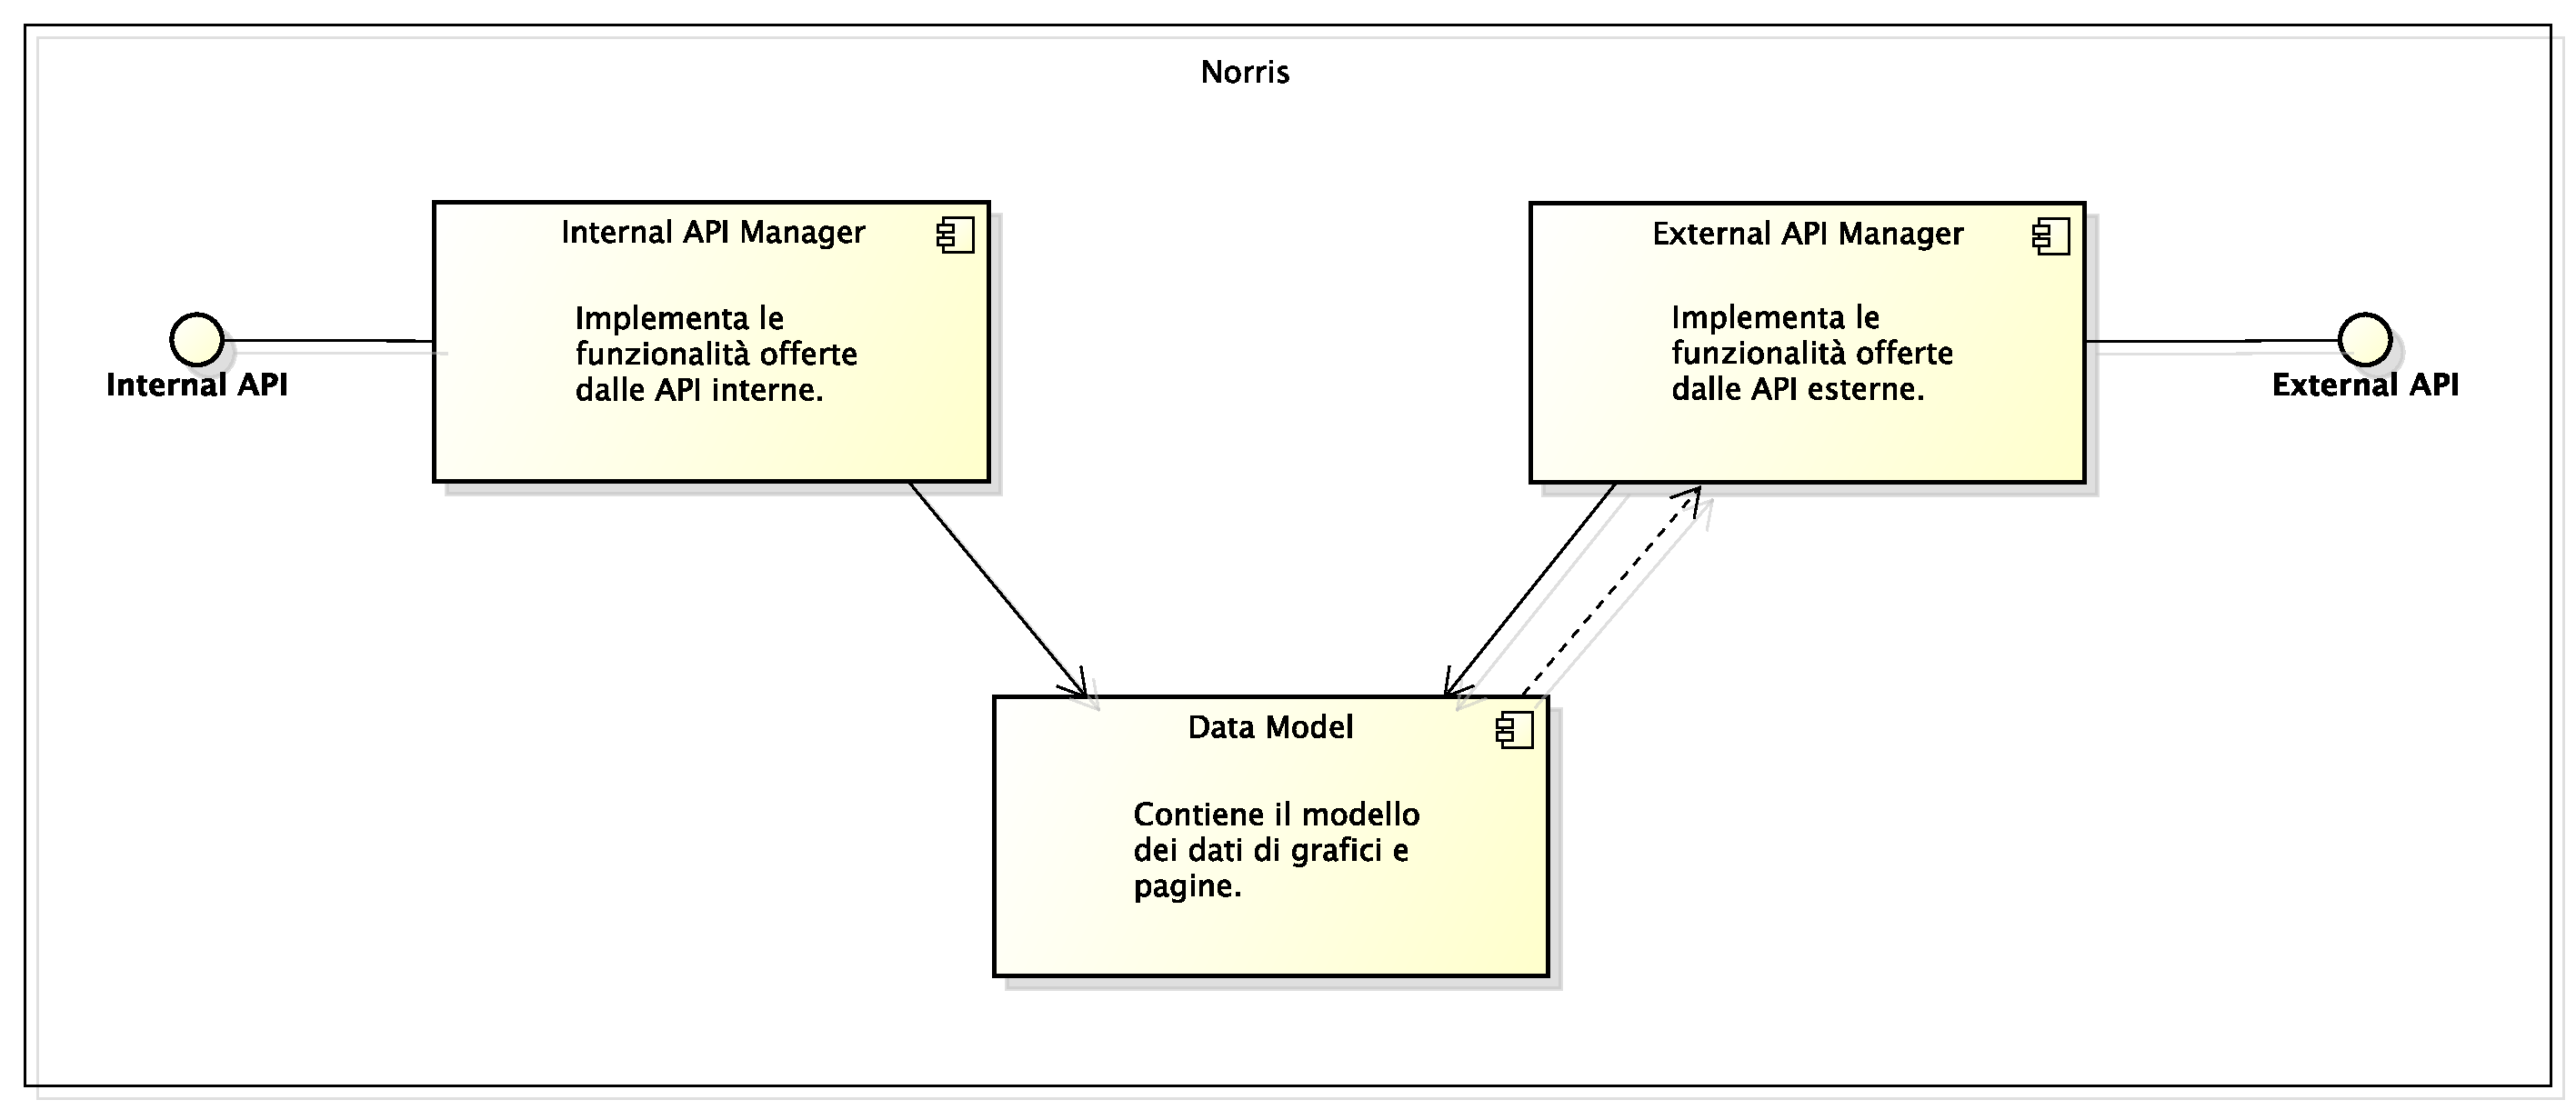
\includegraphics[width=\textwidth]{SpecificaTecnica/Pics/ComponentiNorris}
	        \caption{Diagramma delle componenti di Norris}
	    \end{figure}
    	Di seguito vengono descritti i ruoli e le responsabilità delle varie componenti che sono state individuate durante la progettazione architetturale di Norris.
    	\level{4}{Internal API Manager}
			La componente Internal \insglo{API} Manager rappresenta un controller per le \insglo{API} interne. Essa si occupa di implementare le funzionalità offerte dall'interfaccia delle \insglo{API} interne, ovvero:
			\begin{itemize}
				\item creare nuovi grafici;
				\item aggiornare i grafici;
				\item creare nuove pagine;
				\item aggiungere i grafici all'istanza di \insglo{Norris};
				\item aggiungere le pagine all'istanza di \insglo{Norris};
				\item aggiungere i grafici alle pagine;
				\item scegliere le impostazioni relative a grafici, pagine e istanza;
				\item permette la definizione di funzioni per l'autenticazione.
			\end{itemize}
		Questa componente si occupa, inoltre, di generare in automatico le pagine create all'interno di un'istanza di \insglo{Norris}, a partire dai modelli in essa contenuti.

		\level{4}{Data Model}
			La componente Data Model è un modello che astrae un'istanza di \insglo{Norris}. Al suo interno vi sono le informazioni relative alla struttura di grafici e pagine, assieme alle rispettive impostazioni. Inoltre vengono fissate le regole con le quali grafici e pagine vengono composti assieme per formare un'istanza di \insglo{Norris}. Il Data Model fornisce i metodi per inserire i dati e configurare le impostazioni. Fornisce inoltre dei metodi per ottenere i valori di queste ultime, in modo da poterle riutilizzare per un altro grafico o pagina. Infine, è qui che vengono memorizzate le informazioni inerenti l'autenticazione.

		\level{4}{External API Manager}
			La componente External \insglo{API} Manager rappresenta un controller per le \insglo{API} esterne. Essa implementa le funzionalità offerte dall'interfaccia delle \insglo{API} esterne, ovvero:
			\begin{itemize}
				\item ottenere la lista dei grafici;
				\item ottenere un grafico con relativi aggiornamenti;
				\item effettuare il login;
				\item effettuare il logout.
			\end{itemize}
		Questa componente si occupa, inoltre, di gestire la comunicazione con il \insglo{server} web. Gestisce quindi sia le richieste \insglo{HTTP}, sia la comunicazione tramite un canale \insglo{websocket}.

	\level{3}{Descrizione delle interazioni tra le componenti}

		\level{4}{Internal API Manager - Data Model}
			Quando lo sviluppatore richiama una funzione definita dalle \insglo{API} interne, la componente Internal \insglo{API} Manager effettua le opportune operazioni di lettura/scrittura nel Data Model.

		\level{4}{External API Manager - Data Model}
			Per fornire le funzionalità descritte dalle \insglo{API} esterne, la componente External \insglo{API} Manager interroga il Data Model sullo stato attuale dell'istanza, richiedendo le informazioni in esso contenute.

		\level{4}{Data Model - External API Manager}
			Quando avviene una modifica nel Data Model, una notifica avvisa l'External \insglo{API} Manager di un avvenuto cambiamento nel modello dei dati. In particolare External \insglo{API} Manager viene notificato quando viene creato un nuovo grafico o quando un grafico esistente viene aggiornato.

	\level{3}{Descrizione delle classi di Norris}
		In questa sezione sono presenti le descrizioni di tutte le classi presenti all'interno del \insglo{prodotto} \insglo{Norris}. Queste sono state suddivise in base al componente nelle quali sono contenute.
		\level{1}{Norris}
    \level{2}{Specifica dei componenti}
	Nella presente sezione è stata riportata e documentata la progettazione di dettaglio del \insglo{prodotto} \insglo{Norris}. Si noti che tale progettazione deriva direttamente dalla progettazione architetturale che può essere trovata all'interno del documento \insdoc{Specifica Tecnica v4.00}. I risultati ottenuti sono stati organizzati e presentati secondo la seguente struttura:
	\begin{enumerate}
		\item vengono innanzitutto presentate le varie classi che sono state individuate. Per ognuna di esse si indica il nome, il tipo, l'eventuale astrattezza, la visibilità e il fatto che estenda altre classi oppure no. In aggiunta a ciò, viene presentata una descrizione completa del ruolo e delle responsabilità della classe oltre a una documentazione completa riguardante tutti gli attributi e i metodi presenti all'interno.
		\item in secondo luogo vengono presentati i diagrammi di sequenza, che hanno lo scopo di descrivere scenari (determinate sequenze di azioni in cui tutte le scelte sono già state effettuate). Essi vengono usati per descrivere le relazioni che intercorrono, in termini di messaggi, tra attori, oggetti ed entità del sistema \insglo{Norris}.
	\end{enumerate}
	Le regole che sono state rispettate, gli strumenti che sono stati usati e le procedure che sono state effettuate possono essere trovate all'interno del documento \insdoc{Norme di Progetto v6.00}.
    \level{3}{Classi}
    	In tale sezione sono riportate delle descrizioni dettagliate delle classi individuate all'interno del documento \insdoc{Specifica Tecnica v4.00}. Tali classi sono presentate e organizzate in modo gerarchico, mantenendo una suddivisione per \insglo{package} di appartenenza.
        \level{1}{Norris}
    \level{2}{Specifica dei componenti}
	Nella presente sezione è stata riportata e documentata la progettazione di dettaglio del \insglo{prodotto} \insglo{Norris}. Si noti che tale progettazione deriva direttamente dalla progettazione architetturale che può essere trovata all'interno del documento \insdoc{Specifica Tecnica v4.00}. I risultati ottenuti sono stati organizzati e presentati secondo la seguente struttura:
	\begin{enumerate}
		\item vengono innanzitutto presentate le varie classi che sono state individuate. Per ognuna di esse si indica il nome, il tipo, l'eventuale astrattezza, la visibilità e il fatto che estenda altre classi oppure no. In aggiunta a ciò, viene presentata una descrizione completa del ruolo e delle responsabilità della classe oltre a una documentazione completa riguardante tutti gli attributi e i metodi presenti all'interno.
		\item in secondo luogo vengono presentati i diagrammi di sequenza, che hanno lo scopo di descrivere scenari (determinate sequenze di azioni in cui tutte le scelte sono già state effettuate). Essi vengono usati per descrivere le relazioni che intercorrono, in termini di messaggi, tra attori, oggetti ed entità del sistema \insglo{Norris}.
	\end{enumerate}
	Le regole che sono state rispettate, gli strumenti che sono stati usati e le procedure che sono state effettuate possono essere trovate all'interno del documento \insdoc{Norme di Progetto v6.00}.
    \level{3}{Classi}
    	In tale sezione sono riportate delle descrizioni dettagliate delle classi individuate all'interno del documento \insdoc{Specifica Tecnica v4.00}. Tali classi sono presentate e organizzate in modo gerarchico, mantenendo una suddivisione per \insglo{package} di appartenenza.
        \level{1}{Norris}
    \level{2}{Specifica dei componenti}
	Nella presente sezione è stata riportata e documentata la progettazione di dettaglio del \insglo{prodotto} \insglo{Norris}. Si noti che tale progettazione deriva direttamente dalla progettazione architetturale che può essere trovata all'interno del documento \insdoc{Specifica Tecnica v4.00}. I risultati ottenuti sono stati organizzati e presentati secondo la seguente struttura:
	\begin{enumerate}
		\item vengono innanzitutto presentate le varie classi che sono state individuate. Per ognuna di esse si indica il nome, il tipo, l'eventuale astrattezza, la visibilità e il fatto che estenda altre classi oppure no. In aggiunta a ciò, viene presentata una descrizione completa del ruolo e delle responsabilità della classe oltre a una documentazione completa riguardante tutti gli attributi e i metodi presenti all'interno.
		\item in secondo luogo vengono presentati i diagrammi di sequenza, che hanno lo scopo di descrivere scenari (determinate sequenze di azioni in cui tutte le scelte sono già state effettuate). Essi vengono usati per descrivere le relazioni che intercorrono, in termini di messaggi, tra attori, oggetti ed entità del sistema \insglo{Norris}.
	\end{enumerate}
	Le regole che sono state rispettate, gli strumenti che sono stati usati e le procedure che sono state effettuate possono essere trovate all'interno del documento \insdoc{Norme di Progetto v6.00}.
    \level{3}{Classi}
    	In tale sezione sono riportate delle descrizioni dettagliate delle classi individuate all'interno del documento \insdoc{Specifica Tecnica v4.00}. Tali classi sono presentate e organizzate in modo gerarchico, mantenendo una suddivisione per \insglo{package} di appartenenza.
        \input{Classi/Norris.tex}

    \level{3}{Classi aggiuntive}
        Per quanto riguarda le classi aggiuntive riguardanti che implementano i tipi “ChartSettings” e “ChartUpdate” si faccia riferimento all'appendice \nameref{app:schemi}, nella quale sono presenti gli schemi \insglo{JSON} di tali oggetti.
        \input{Classi/NorrisAggiuntive.tex}

    \level{2}{Diagrammi di sequenza}
    	In tale sezione vengono presentati i diagrammi di sequenza, che hanno lo scopo di descrivere scenari (determinate sequenze di azioni in cui tutte le scelte sono già state effettuate). Essi vengono usati per descrivere le relazioni che intercorrono, in termini di messaggi, tra attori, oggetti ed entità del sistema \insglo{Norris}.
        \level{3}{Creazione di un chart}
        	Tale diagramma descrive come viene creato un chart di un certo tipo prefissato.
            \begin{figure}[H]
                \centering
                \includegraphics[scale=0.3]{DefinizioneDiProdotto/Pics/NorrisCreazioneChart}
                \caption{Diagramma di sequenza - Norris, creazione chart}
            \end{figure}


        \level{3}{Aggiornamento di un chart}
        	Tale diagramma descrive come viene aggiornato un chart di un certo tipo (sulla base delle modalità di aggiornamento definite per quel tipo di grafico).
            \begin{figure}[H]
                \centering
                \includegraphics[scale=0.3]{DefinizioneDiProdotto/Pics/NorrisAggiornamentoChart}
                \caption{Diagramma di sequenza - Norris, aggiornamento chart}
            \end{figure}

            
        \level{3}{Invio lista dei grafici}
        	Tale diagramma descrive come viene gestita la richiesta della lista di tutti i grafici contenuti in una certa istanza di \insglo{Norris}.
            \begin{figure}[H]
                \centering
                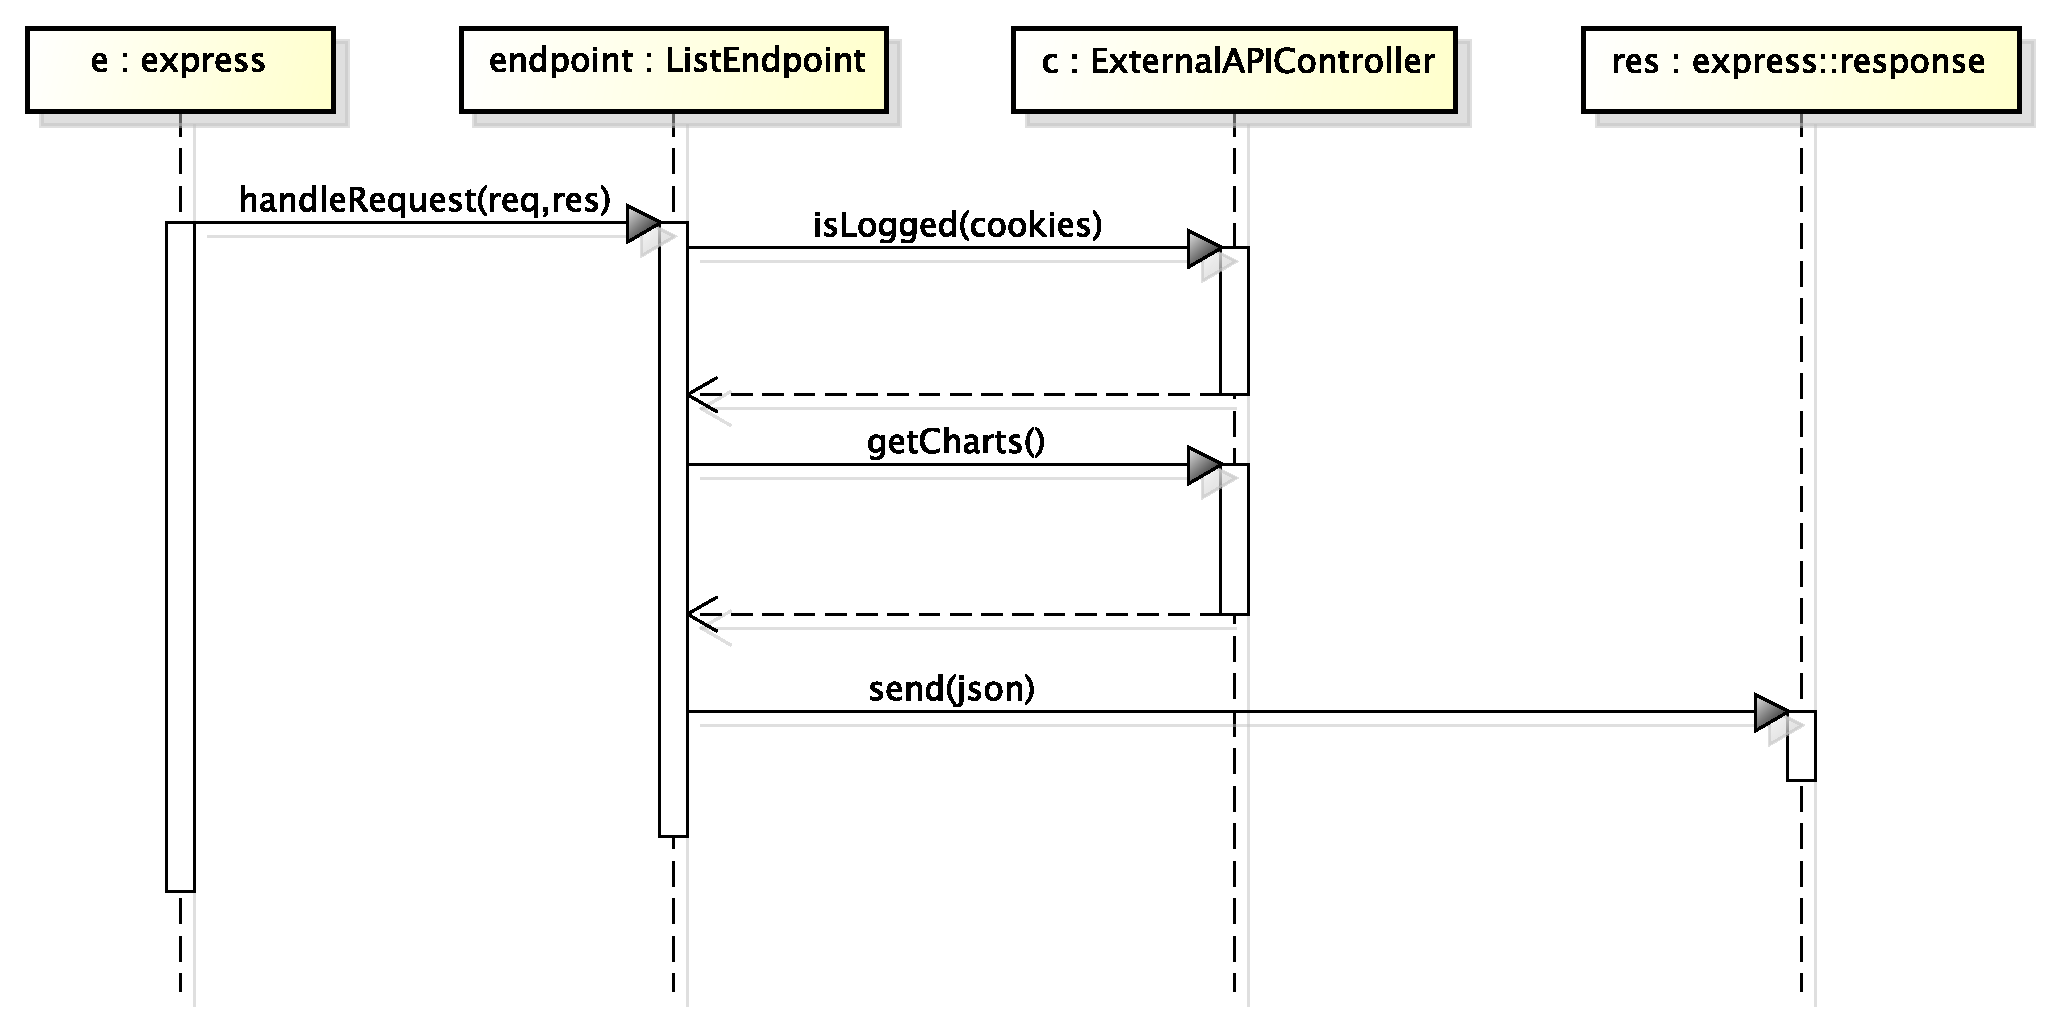
\includegraphics[scale=0.3]{DefinizioneDiProdotto/Pics/NorrisInvioLista}
                \caption{Diagramma di sequenza - Norris, invio lista}
            \end{figure}

            
        \level{3}{Invio di un chart}
        	Tale diagramma descrive come viene gestita la richiesta di un chart da parte di un \insglo{client} dal sistema \insglo{Norris}.
            \begin{figure}[H]
                \centering
                \includegraphics[scale=0.3]{DefinizioneDiProdotto/Pics/NorrisInvioChart}
                \caption{Diagramma di sequenza - Norris, invio chart}
            \end{figure}


    \level{3}{Classi aggiuntive}
        Per quanto riguarda le classi aggiuntive riguardanti che implementano i tipi “ChartSettings” e “ChartUpdate” si faccia riferimento all'appendice \nameref{app:schemi}, nella quale sono presenti gli schemi \insglo{JSON} di tali oggetti.
        
			\level{4}[NorrisSettingsImpl]{NorrisAggiuntive::NorrisSettingsImpl}
			

		\IfFileExists{DefinizioneDiProdotto/Pics/ClassiAggiuntive/NorrisSettingsImpl.pdf}{
			\begin{figure}[H]
				\centering
				\includegraphics[scale=0.5]{DefinizioneDiProdotto/Pics/ClassiAggiuntive/NorrisSettingsImpl}
				\caption{NorrisSettingsImpl}
			\end{figure}
		}
	
			
			\begin{itemize}
			\item \textbf{Nome:} NorrisSettingsImpl
			\item \textbf{Tipo:} classe
			
		\item \textbf{Astratta:}
		no
			\item \textbf{Visibilità:} public
			\item \textbf{Descrizione:} La classe NorrisSettingsImpl definisce le impostazioni relative ad un'istanza di Norris. Lo sviluppatore può definire le funzioni che verranno eseguite per l'autenticazione.
			\item \textbf{Attributi:}
				\begin{itemize}
				\setlength{\itemsep}{5pt}
				
					\item[\ding{111}] {+login : Function} \\ [1mm] L'attributo login rappresenta la funzione che verrà eseguita per avviare la sessione di un utente.
					\item[\ding{111}] {+logout : Function} \\ [1mm] L'attributo login rappresenta la funzione che verrà eseguita per terminare la sessione di un utente.
					\item[\ding{111}] {+keepAlive : Function} \\ [1mm] L'attributo login rappresenta la funzione che verrà eseguita per rinnovare la sessione di un utente.
					\item[\ding{111}] {+isLogged : Function} \\ [1mm] L'attributo login rappresenta la funzione che verrà eseguita per verificare lo stato dela sessione di un utente.
					\item[\ding{111}] {+endpoint : String} \\ [1mm] L'attributo endpoint definisce il path al quale sono disponibili le API esterne.
					\item[\ding{111}] {+secret : String} \\ [1mm] L'attributo secret definisce la chiave di cifrature per i cookie firmati.
					\item[\ding{111}] {+origins : String[]} \\ [1mm] L'attributo origin definisce gli host attendibili, verso i quali saranno disponibili le API esterne.
				\end{itemize}
		
			\end{itemize}
	
			\level{4}[PageSettingsImpl]{NorrisAggiuntive::PageSettingsImpl}
			

		\IfFileExists{DefinizioneDiProdotto/Pics/ClassiAggiuntive/PageSettingsImpl.pdf}{
			\begin{figure}[H]
				\centering
				\includegraphics[scale=0.5]{DefinizioneDiProdotto/Pics/ClassiAggiuntive/PageSettingsImpl}
				\caption{PageSettingsImpl}
			\end{figure}
		}
	
			
			\begin{itemize}
			\item \textbf{Nome:} PageSettingsImpl
			\item \textbf{Tipo:} classe
			
		\item \textbf{Astratta:}
		no
			\item \textbf{Visibilità:} public
			\item \textbf{Descrizione:} La classe PageSettingsImpl definisce le impostazioni di una pagina di Norris.
			\item \textbf{Attributi:}
				\begin{itemize}
				\setlength{\itemsep}{5pt}
				
					\item[\ding{111}] {+title : String} \\ [1mm] L'attributo title rappresenta il titolo di una pagina di Norris.
					\item[\ding{111}] {+maxChartsRow : int} \\ [1mm] L'attributo title rappresenta il numero massimo di righe visualizzabili all'interno della pagina.
					\item[\ding{111}] {+maxChartsCol : int} \\ [1mm] L'attributo title rappresenta il numero massimo di colonne visualizzabili all'interno della pagina.
				\end{itemize}
		
			\end{itemize}
	

    \level{2}{Diagrammi di sequenza}
    	In tale sezione vengono presentati i diagrammi di sequenza, che hanno lo scopo di descrivere scenari (determinate sequenze di azioni in cui tutte le scelte sono già state effettuate). Essi vengono usati per descrivere le relazioni che intercorrono, in termini di messaggi, tra attori, oggetti ed entità del sistema \insglo{Norris}.
        \level{3}{Creazione di un chart}
        	Tale diagramma descrive come viene creato un chart di un certo tipo prefissato.
            \begin{figure}[H]
                \centering
                \includegraphics[scale=0.3]{DefinizioneDiProdotto/Pics/NorrisCreazioneChart}
                \caption{Diagramma di sequenza - Norris, creazione chart}
            \end{figure}


        \level{3}{Aggiornamento di un chart}
        	Tale diagramma descrive come viene aggiornato un chart di un certo tipo (sulla base delle modalità di aggiornamento definite per quel tipo di grafico).
            \begin{figure}[H]
                \centering
                \includegraphics[scale=0.3]{DefinizioneDiProdotto/Pics/NorrisAggiornamentoChart}
                \caption{Diagramma di sequenza - Norris, aggiornamento chart}
            \end{figure}

            
        \level{3}{Invio lista dei grafici}
        	Tale diagramma descrive come viene gestita la richiesta della lista di tutti i grafici contenuti in una certa istanza di \insglo{Norris}.
            \begin{figure}[H]
                \centering
                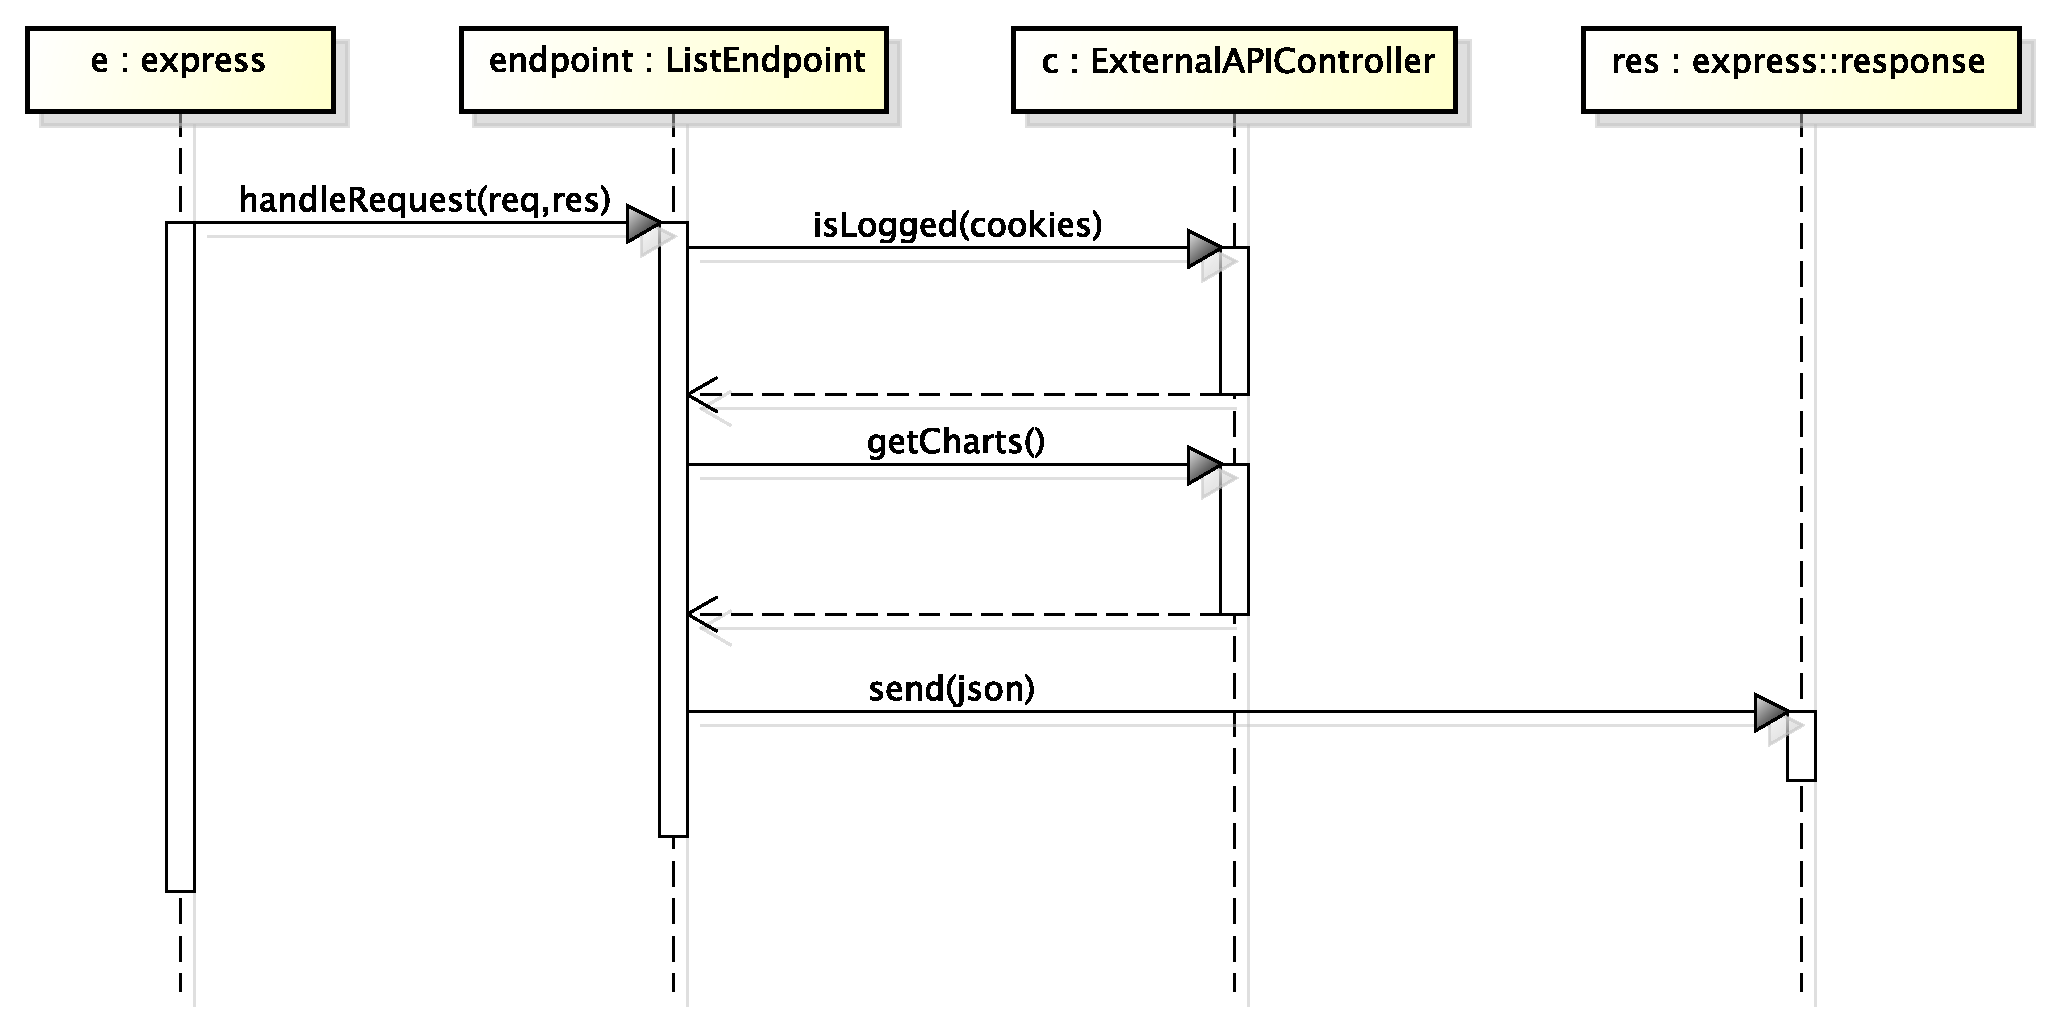
\includegraphics[scale=0.3]{DefinizioneDiProdotto/Pics/NorrisInvioLista}
                \caption{Diagramma di sequenza - Norris, invio lista}
            \end{figure}

            
        \level{3}{Invio di un chart}
        	Tale diagramma descrive come viene gestita la richiesta di un chart da parte di un \insglo{client} dal sistema \insglo{Norris}.
            \begin{figure}[H]
                \centering
                \includegraphics[scale=0.3]{DefinizioneDiProdotto/Pics/NorrisInvioChart}
                \caption{Diagramma di sequenza - Norris, invio chart}
            \end{figure}


    \level{3}{Classi aggiuntive}
        Per quanto riguarda le classi aggiuntive riguardanti che implementano i tipi “ChartSettings” e “ChartUpdate” si faccia riferimento all'appendice \nameref{app:schemi}, nella quale sono presenti gli schemi \insglo{JSON} di tali oggetti.
        
			\level{4}[NorrisSettingsImpl]{NorrisAggiuntive::NorrisSettingsImpl}
			

		\IfFileExists{DefinizioneDiProdotto/Pics/ClassiAggiuntive/NorrisSettingsImpl.pdf}{
			\begin{figure}[H]
				\centering
				\includegraphics[scale=0.5]{DefinizioneDiProdotto/Pics/ClassiAggiuntive/NorrisSettingsImpl}
				\caption{NorrisSettingsImpl}
			\end{figure}
		}
	
			
			\begin{itemize}
			\item \textbf{Nome:} NorrisSettingsImpl
			\item \textbf{Tipo:} classe
			
		\item \textbf{Astratta:}
		no
			\item \textbf{Visibilità:} public
			\item \textbf{Descrizione:} La classe NorrisSettingsImpl definisce le impostazioni relative ad un'istanza di Norris. Lo sviluppatore può definire le funzioni che verranno eseguite per l'autenticazione.
			\item \textbf{Attributi:}
				\begin{itemize}
				\setlength{\itemsep}{5pt}
				
					\item[\ding{111}] {+login : Function} \\ [1mm] L'attributo login rappresenta la funzione che verrà eseguita per avviare la sessione di un utente.
					\item[\ding{111}] {+logout : Function} \\ [1mm] L'attributo login rappresenta la funzione che verrà eseguita per terminare la sessione di un utente.
					\item[\ding{111}] {+keepAlive : Function} \\ [1mm] L'attributo login rappresenta la funzione che verrà eseguita per rinnovare la sessione di un utente.
					\item[\ding{111}] {+isLogged : Function} \\ [1mm] L'attributo login rappresenta la funzione che verrà eseguita per verificare lo stato dela sessione di un utente.
					\item[\ding{111}] {+endpoint : String} \\ [1mm] L'attributo endpoint definisce il path al quale sono disponibili le API esterne.
					\item[\ding{111}] {+secret : String} \\ [1mm] L'attributo secret definisce la chiave di cifrature per i cookie firmati.
					\item[\ding{111}] {+origins : String[]} \\ [1mm] L'attributo origin definisce gli host attendibili, verso i quali saranno disponibili le API esterne.
				\end{itemize}
		
			\end{itemize}
	
			\level{4}[PageSettingsImpl]{NorrisAggiuntive::PageSettingsImpl}
			

		\IfFileExists{DefinizioneDiProdotto/Pics/ClassiAggiuntive/PageSettingsImpl.pdf}{
			\begin{figure}[H]
				\centering
				\includegraphics[scale=0.5]{DefinizioneDiProdotto/Pics/ClassiAggiuntive/PageSettingsImpl}
				\caption{PageSettingsImpl}
			\end{figure}
		}
	
			
			\begin{itemize}
			\item \textbf{Nome:} PageSettingsImpl
			\item \textbf{Tipo:} classe
			
		\item \textbf{Astratta:}
		no
			\item \textbf{Visibilità:} public
			\item \textbf{Descrizione:} La classe PageSettingsImpl definisce le impostazioni di una pagina di Norris.
			\item \textbf{Attributi:}
				\begin{itemize}
				\setlength{\itemsep}{5pt}
				
					\item[\ding{111}] {+title : String} \\ [1mm] L'attributo title rappresenta il titolo di una pagina di Norris.
					\item[\ding{111}] {+maxChartsRow : int} \\ [1mm] L'attributo title rappresenta il numero massimo di righe visualizzabili all'interno della pagina.
					\item[\ding{111}] {+maxChartsCol : int} \\ [1mm] L'attributo title rappresenta il numero massimo di colonne visualizzabili all'interno della pagina.
				\end{itemize}
		
			\end{itemize}
	

    \level{2}{Diagrammi di sequenza}
    	In tale sezione vengono presentati i diagrammi di sequenza, che hanno lo scopo di descrivere scenari (determinate sequenze di azioni in cui tutte le scelte sono già state effettuate). Essi vengono usati per descrivere le relazioni che intercorrono, in termini di messaggi, tra attori, oggetti ed entità del sistema \insglo{Norris}.
        \level{3}{Creazione di un chart}
        	Tale diagramma descrive come viene creato un chart di un certo tipo prefissato.
            \begin{figure}[H]
                \centering
                \includegraphics[scale=0.3]{DefinizioneDiProdotto/Pics/NorrisCreazioneChart}
                \caption{Diagramma di sequenza - Norris, creazione chart}
            \end{figure}


        \level{3}{Aggiornamento di un chart}
        	Tale diagramma descrive come viene aggiornato un chart di un certo tipo (sulla base delle modalità di aggiornamento definite per quel tipo di grafico).
            \begin{figure}[H]
                \centering
                \includegraphics[scale=0.3]{DefinizioneDiProdotto/Pics/NorrisAggiornamentoChart}
                \caption{Diagramma di sequenza - Norris, aggiornamento chart}
            \end{figure}

            
        \level{3}{Invio lista dei grafici}
        	Tale diagramma descrive come viene gestita la richiesta della lista di tutti i grafici contenuti in una certa istanza di \insglo{Norris}.
            \begin{figure}[H]
                \centering
                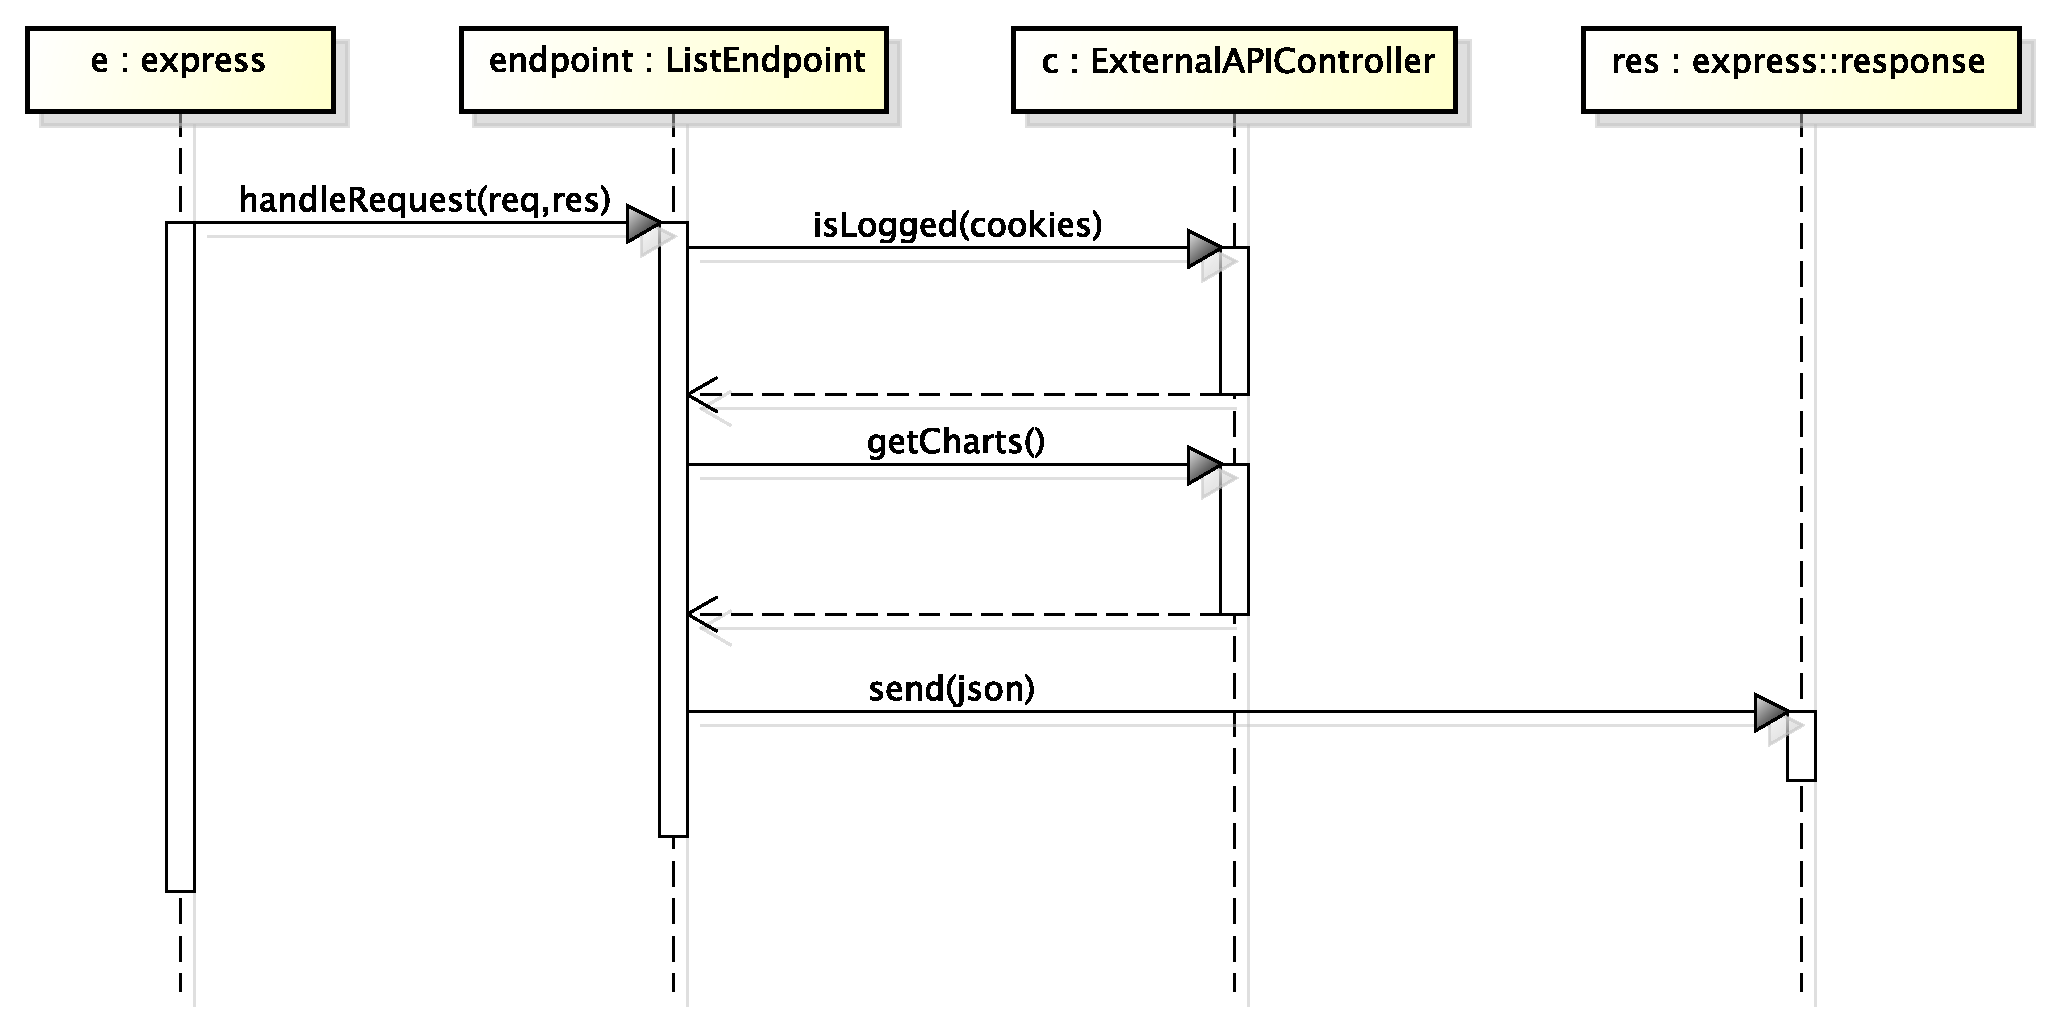
\includegraphics[scale=0.3]{DefinizioneDiProdotto/Pics/NorrisInvioLista}
                \caption{Diagramma di sequenza - Norris, invio lista}
            \end{figure}

            
        \level{3}{Invio di un chart}
        	Tale diagramma descrive come viene gestita la richiesta di un chart da parte di un \insglo{client} dal sistema \insglo{Norris}.
            \begin{figure}[H]
                \centering
                \includegraphics[scale=0.3]{DefinizioneDiProdotto/Pics/NorrisInvioChart}
                \caption{Diagramma di sequenza - Norris, invio chart}
            \end{figure}

		\level{4}{Classi aggiuntive Norris}
	Le interfacce \insglo{Norris}::DataModel::ChartData, \insglo{Norris}::DataModel::ChartSettings e \insglo{Norris}::DataModel::ChartUpdate rappresentano genericamente i vari oggetti che utilizzeremo per rappresentare i dati, le impostazioni e gli aggiornamamenti. Tali oggetti sono nel formato \insglo{JSON} ed essendo molto numerosi abbiamo deciso di non inserirle nel diagramma ma di elencarle e descriverle di seguito.

	\begin{itemize}
		\item \textbf{Norris::DataModel::NorrisChart::BarChartData} Questa classe implementa l'interfaccia \insglo{Norris}::DataModel::ChartData. Essa si occupa di rappresentare i dati di un grafico \insglo{bar chart};

		\item \textbf{\insglo{Norris}::DataModel::NorrisChart::LineChartData} Questa classe implementa l'interfaccia \insglo{Norris}::DataModel::ChartData. Essa si occupa di rappresentare i dati di un grafico \insglo{line chart};

		\item \textbf{\insglo{Norris}::DataModel::NorrisChart::MapChartData} Questa classe implementa l'interfaccia \insglo{Norris}::DataModel::ChartData. Essa si occupa di rappresentare i dati di un grafico \insglo{map chart};

		\item \textbf{\insglo{Norris}::DataModel::NorrisChart::TableData} Questa classe implementa l'interfaccia \linebreak \insglo{Norris}::DataModel::ChartData. Essa si occupa di rappresentare i dati di un grafico \insglo{table};

		\item \textbf{\insglo{Norris}::DataModel::NorrisChart::BarChartSetting} Questa classe implementa l'interfaccia \insglo{Norris}::DataModel::ChartSettings. Essa rappresenta le impostazioni di un grafico di tipo \insglo{bar chart};

		\item \textbf{\insglo{Norris}::DataModel::NorrisChart::LineChartSetting} Questa classe implementa l'interfaccia \insglo{Norris}::DataModel::ChartSettings. Essa rappresenta le impostazioni di un grafico di tipo \insglo{line chart};

		\item \textbf{\insglo{Norris}::DataModel::NorrisChart::MapChartSetting} Questa classe implementa l'interfaccia \insglo{Norris}::DataModel::ChartSettings. Essa rappresenta le impostazioni di un grafico di tipo \insglo{map chart};

		\item \textbf{\insglo{Norris}::DataModel::NorrisChart::TableSetting} Questa classe implementa l'interfaccia \insglo{Norris}::DataModel::ChartSettings. Essa rappresenta le impostazioni di un grafico di tipo \insglo{table};

		\item \textbf{\insglo{Norris}::DataModel::NorrisChart::BarChartInPlaceUpdate} Questa classe implementa l'interfaccia \insglo{Norris}::DataModel::ChartUpdate. Essa rappresenta un pacchetto di aggiornamento di tipo \insglo{in place} per un grafico di tipo \insglo{bar chart};

		\item \textbf{\insglo{Norris}::DataModel::NorrisChart::LineChartInPlaceUpdate} Questa classe implementa l'interfaccia \insglo{Norris}::DataModel::ChartUpdate. Essa rappresenta un pacchetto di aggiornamento di tipo \insglo{in place} per un grafico di tipo \insglo{line chart};

		\item \textbf{\insglo{Norris}::DataModel::NorrisChart::LineChartStreamUpdate} Questa classe implementa l'interfaccia \insglo{Norris}::DataModel::ChartUpdate. Essa rappresenta un pacchetto di aggiornamento di tipo \insglo{stream} per un grafico di tipo \insglo{line chart};

		\item \textbf{\insglo{Norris}::DataModel::NorrisChart::MapChartInPlaceUpdate} Questa classe implementa l'interfaccia \insglo{Norris}::DataModel::ChartUpdate. Essa rappresenta un pacchetto di aggiornamento di tipo \insglo{in place} per un grafico di tipo \insglo{map chart};

		\item \textbf{\insglo{Norris}::DataModel::NorrisChart::MapChartMovieUpdate} Questa classe implementa l'interfaccia \insglo{Norris}::DataModel::ChartUpdate. Essa rappresenta un pacchetto di aggiornamento di tipo \insglo{movie} per un grafico di tipo \insglo{map chart};

		\item \textbf{\insglo{Norris}::DataModel::NorrisChart::TableStreamUpdate} Questa classe implementa l'interfaccia \insglo{Norris}::DataModel::ChartUpdate. Essa rappresenta un pacchetto di aggiornamento di tipo \insglo{stream} per un grafico di tipo \insglo{table};

		\item \textbf{\insglo{Norris}::DataModel::NorrisChart::TableInPlaceUpdate} Questa classe implementa l'interfaccia \insglo{Norris}::DataModel::ChartUpdate. Essa rappresenta un pacchetto di aggiornamento di tipo \insglo{in place} per un grafico di tipo \insglo{table}.
	\end{itemize}

	\level{3}{Interazioni tra classi dei componenti di Norris}
	Il seguente diagramma UML rappresenta le interazioni tra le classi dei vari componenti di Norris.\\
	Alcune classi non sono state volontariamente inserite per rendere più comprendibile il diagramma.
	\begin{figure}[H]\centering
		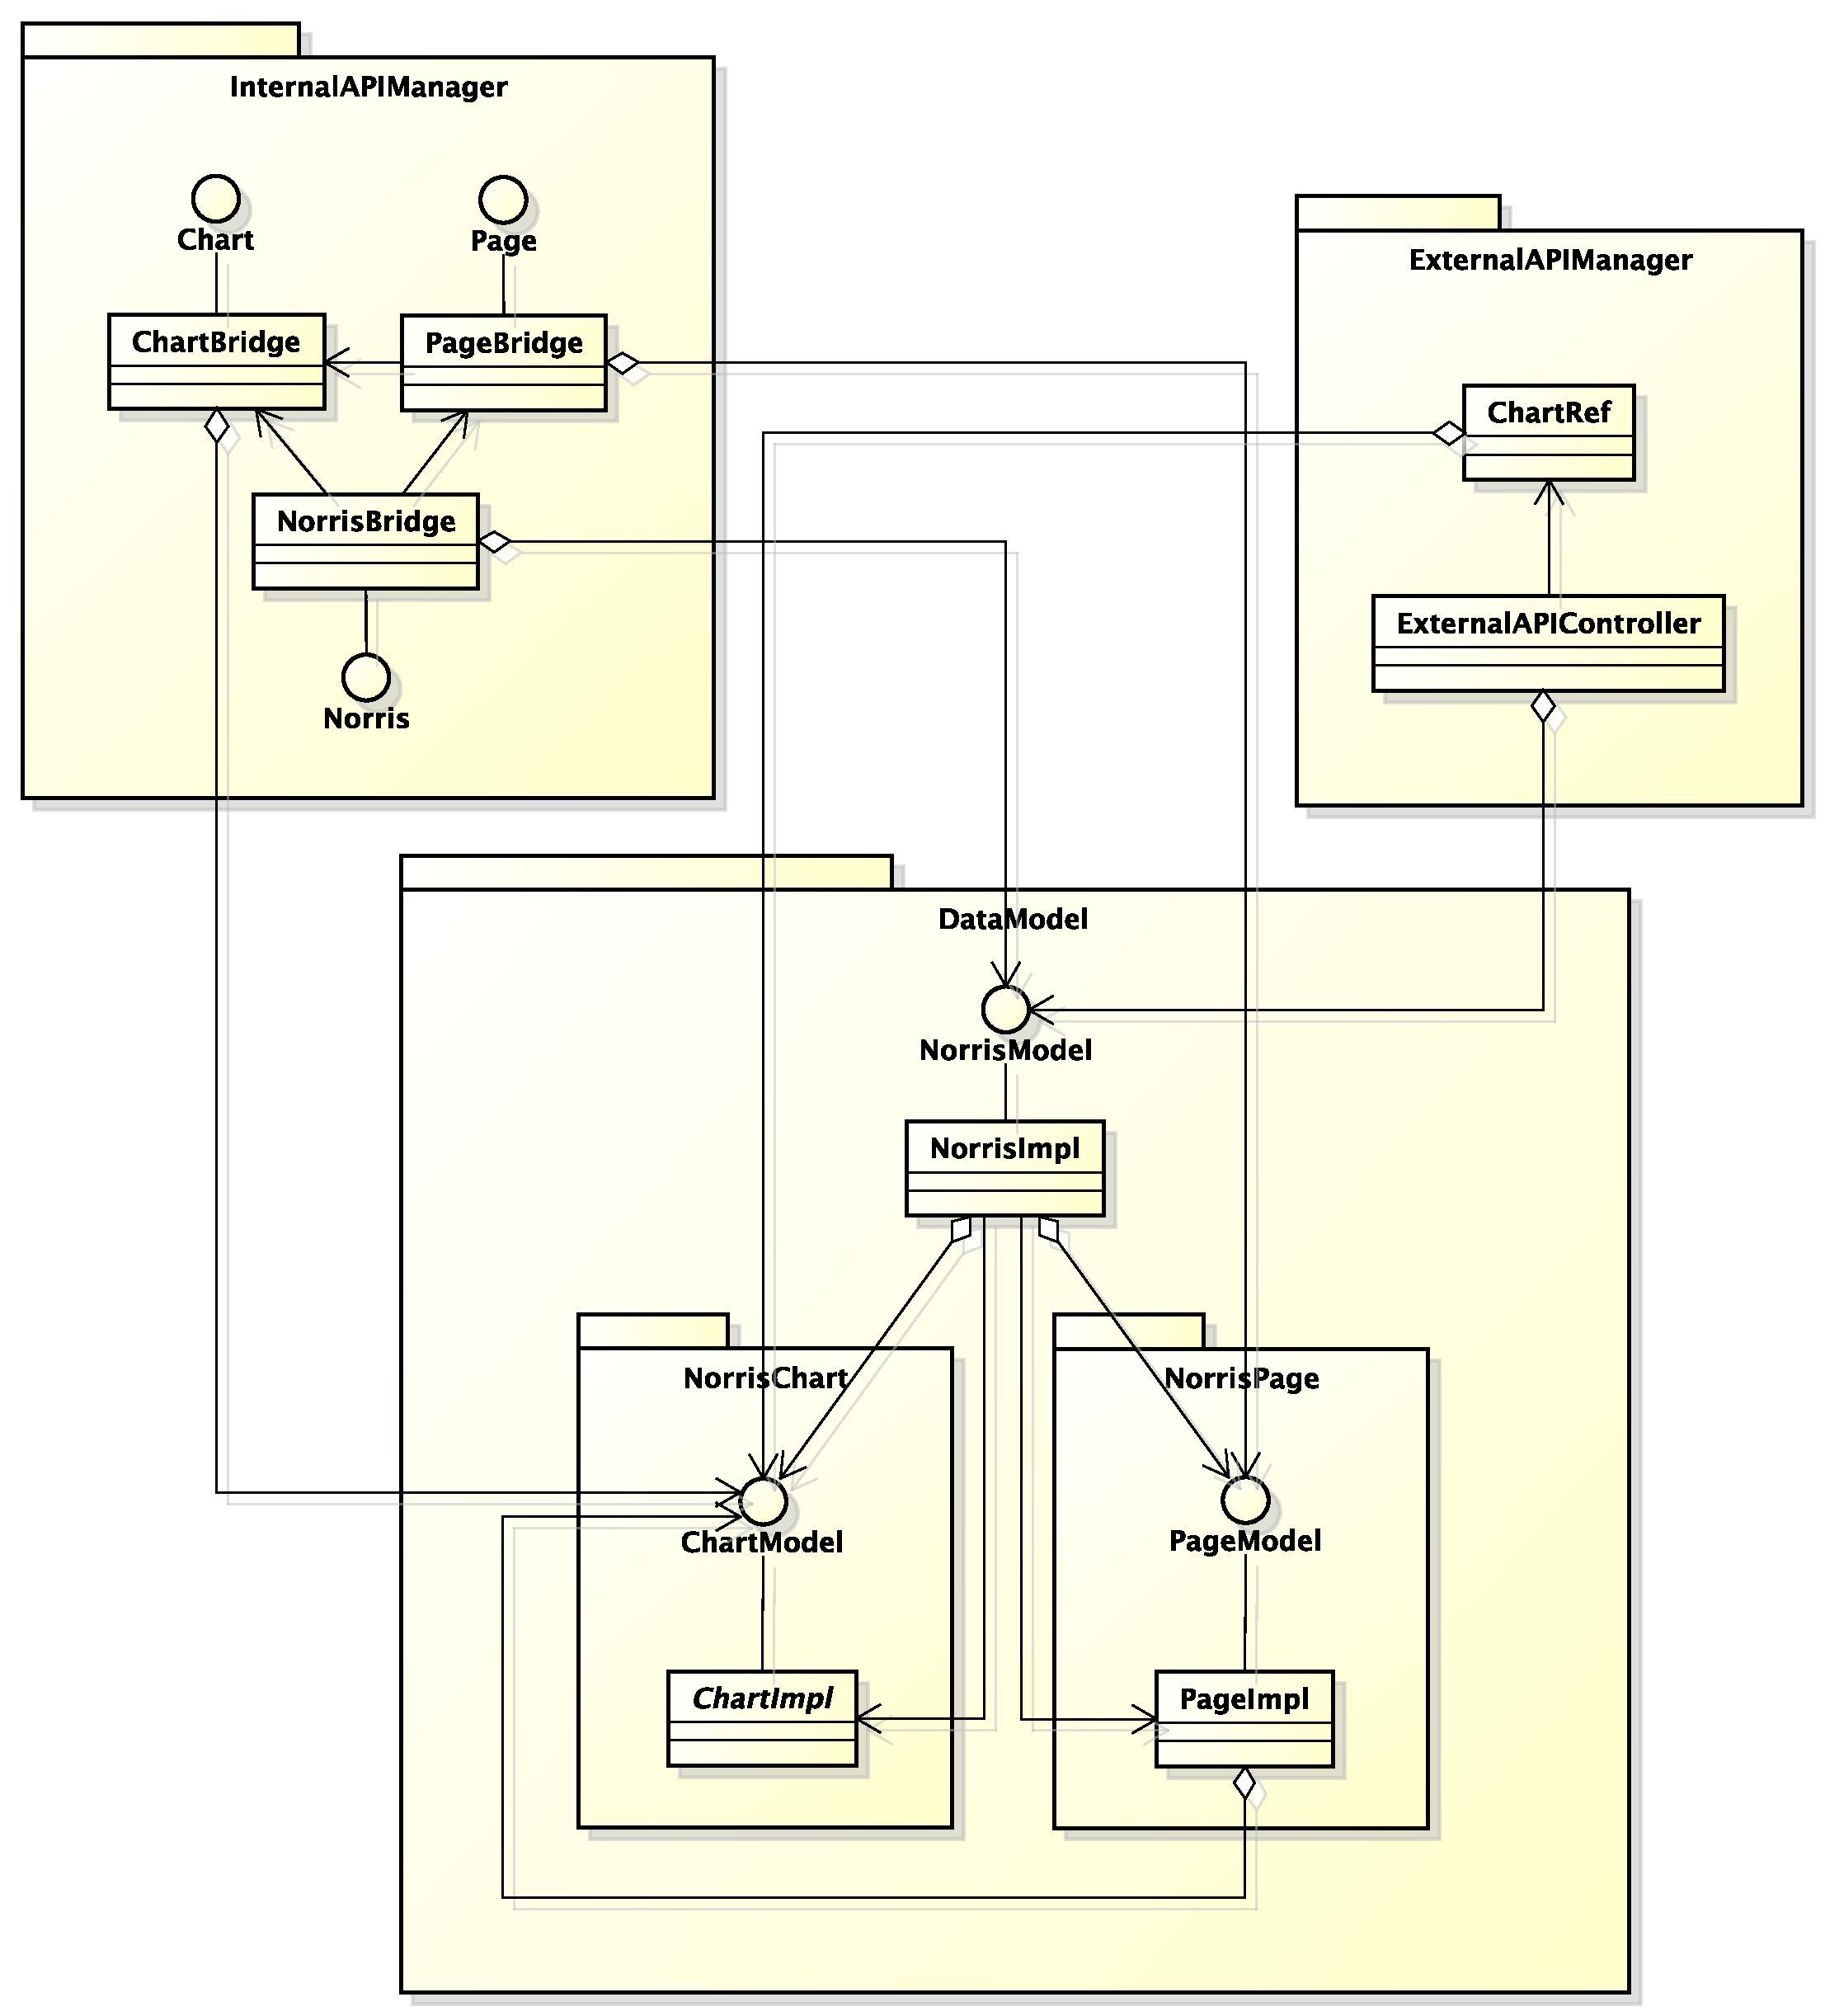
\includegraphics[width=\textwidth]{SpecificaTecnica/Pics/InterazioniComponentiNorris.pdf}
		\caption{Diagramma delle interazioni tra classi di componenti di Norris}
	\end{figure}

	\level{3}{Design pattern utilizzati con le classi}
		Nella progettazione delle classi di \insglo{Norris} abbiamo deciso di utilizzare alcuni \insglo{design pattern}. Riportiamo di seguito una loro breve descrizione e il contesto nel quale sono stati utilizzati.
		
		\level{4}{Bridge}
			Il Bridge è un \insglo{pattern} strutturale pensato per separare l'interfaccia di una classe dalla sua implementazione. In particolare, utilizza i concetti di \textit{encapsulation}, \textit{aggregation} ed \textit{inheritance} per separare varie responsabilità in classi differenti. \\
			Il \insglo{design pattern} Bridge si differenzia dal \insglo{pattern} Adapter, in quanto il primo viene utilizzato fin dall'inizio della progettazione per consentire ad astrazioni ed implementazioni di variare in modo indipendente, mentre il secondo viene usato quando si vogliono adattare classi inizialmente non correlate e viene introdotto dopo che queste sono state progettate.
			Per una descrizione più approfondita del \insglo{pattern} e dei vantaggi derivanti dalla sua applicazione si rimanda all'appendice \nameref{app:bridge}.
			\level{5}{Contesto di utilizzo}
				In \insglo{Norris} questo \insglo{pattern} viene utilizzato nel \insglo{package} InternalAPIManager per separare l'implementazione dei chart (presente nel \insglo{package} DataModel) dall'interfaccia fornita allo sviluppatore. Viene inoltre utilizzato nel package ExteralAPIManger.
				\begin{figure}[H]\centering
	        		\includegraphics[width=\textwidth]{SpecificaTecnica/Pics/DesignPatternNorris/Bridge1}
	        		\caption{Bridge pattern in Norris}
	    		\end{figure}
	    		\begin{figure}[H]\centering
	        		\includegraphics[width=\textwidth]{SpecificaTecnica/Pics/DesignPatternNorris/Bridge2}
	        		\caption{Bridge pattern in Norris}
	    		\end{figure}	
				
		\level{4}{Dependency Injection}
			Dependency Injection è un \insglo{pattern} architetturale il cui scopo è separare il comportamento di una componente dalla risoluzione delle sue dipendenze.\\
			Per la descrizione del \insglo{pattern} e dei vantaggi derivanti dalla sua applicazione si rimanda all'appendice \nameref{app:dependencyinjection}.
			\level{5}{Contesto di utilizzo}
				Il \insglo{pattern} Dependency Injection viene utilizzato con le classi che implementano le seguenti interfacce:
				\begin{itemize}
					\item ExternalAPIManager::EndpointFactory, inietta in ExternalAPIManager::ExternalAPIController le dipendenze verso i diversi Endpoint;
					\item DataModel::ChartFactory, inietta in DataModel::ChartImpl le  corrispondenze tra i tipi di grafico e le rispettive classi factory;
					\item DataModel::Updater, inietta in DataModel::ChartImpl le corrispondenze tra i diversi tipi di aggiornamenti e le classi che li implementano.
				\end{itemize}
				
				\level{4}{Factory Method}
				Il \insglo{pattern} creazionale Factory Method si occupa di fornire un'interfaccia per la creazione di famiglie di prodotti, senza dover specificare classi concrete.\\
		Per la descrizione del \insglo{pattern} e dei vantaggi derivanti dalla sua applicazione si rimanda all'appendice \nameref{app:abstractfactory}.
					\level{5}{Contesto di utilizzo}
					Gli elementi che implementano Factory Method sono quelli indicati in seguito.
					\begin{itemize}
						\item Interfacce:
						\begin{itemize}
							\item ChartFactory, con cui vengono generati i diversi tipi di grafici;
							\item ExternalAPIManager::EndpointFactory, con cui sono generati i diversi tipi di controller dei grafici.
						\end{itemize}
						\item Classi:
						\begin{itemize}
							\item DataModel::BarChartFactory;
							\item DataModel::LineChartFactory;
							\item DataModel::MapChartFactory;
							\item DataModel::TableFactory;
							\item ExternalAPIManager::ChartEndpointFactory;
							\item ExternalAPIManager::AuthenticationEndpointFactory;
							\item ExternalAPIManager::ListEndpointFactory.
						\end{itemize}
					\end{itemize}
					\begin{figure}[H]\centering
	        		\includegraphics[width=\textwidth]{SpecificaTecnica/Pics/DesignPatternNorris/Factory1}
	        		\caption{Factory Method pattern in Norris}
	    			\end{figure}
	    			\begin{figure}[H]\centering
	        			\includegraphics[width=\textwidth]{SpecificaTecnica/Pics/DesignPatternNorris/Factory2}
	        			\caption{Factory Method pattern in Norris}
	    			\end{figure}
			
				\level{4}{Observer}
			L'Observer è un \insglo{pattern} comportamentale che ha lo scopo di monitorare lo stato di diversi oggetti legati ad un soggetto.
			Per la descrizione del \insglo{pattern} e dei vantaggi derivanti dalla sua applicazione si rimanda all'appendice \nameref{app:observer}.
			\level{5}{Contesto di utilizzo}	    	
				Il \insglo{pattern} Observer si basa sugli oggetti “osservabili” e sugli “osservatori”.\\
				Le interfacce che che estendono Observable sono le seguenti:
				\begin{itemize}
					\item DataModel::ChartModel;
					\item DataModel::NorrisModel.
				\end{itemize}
				L'interfaccia Observer è implementata dalla classe EventEmitter fornita da \insglo{Node.js}.
				\begin{figure}[H]\centering
	        		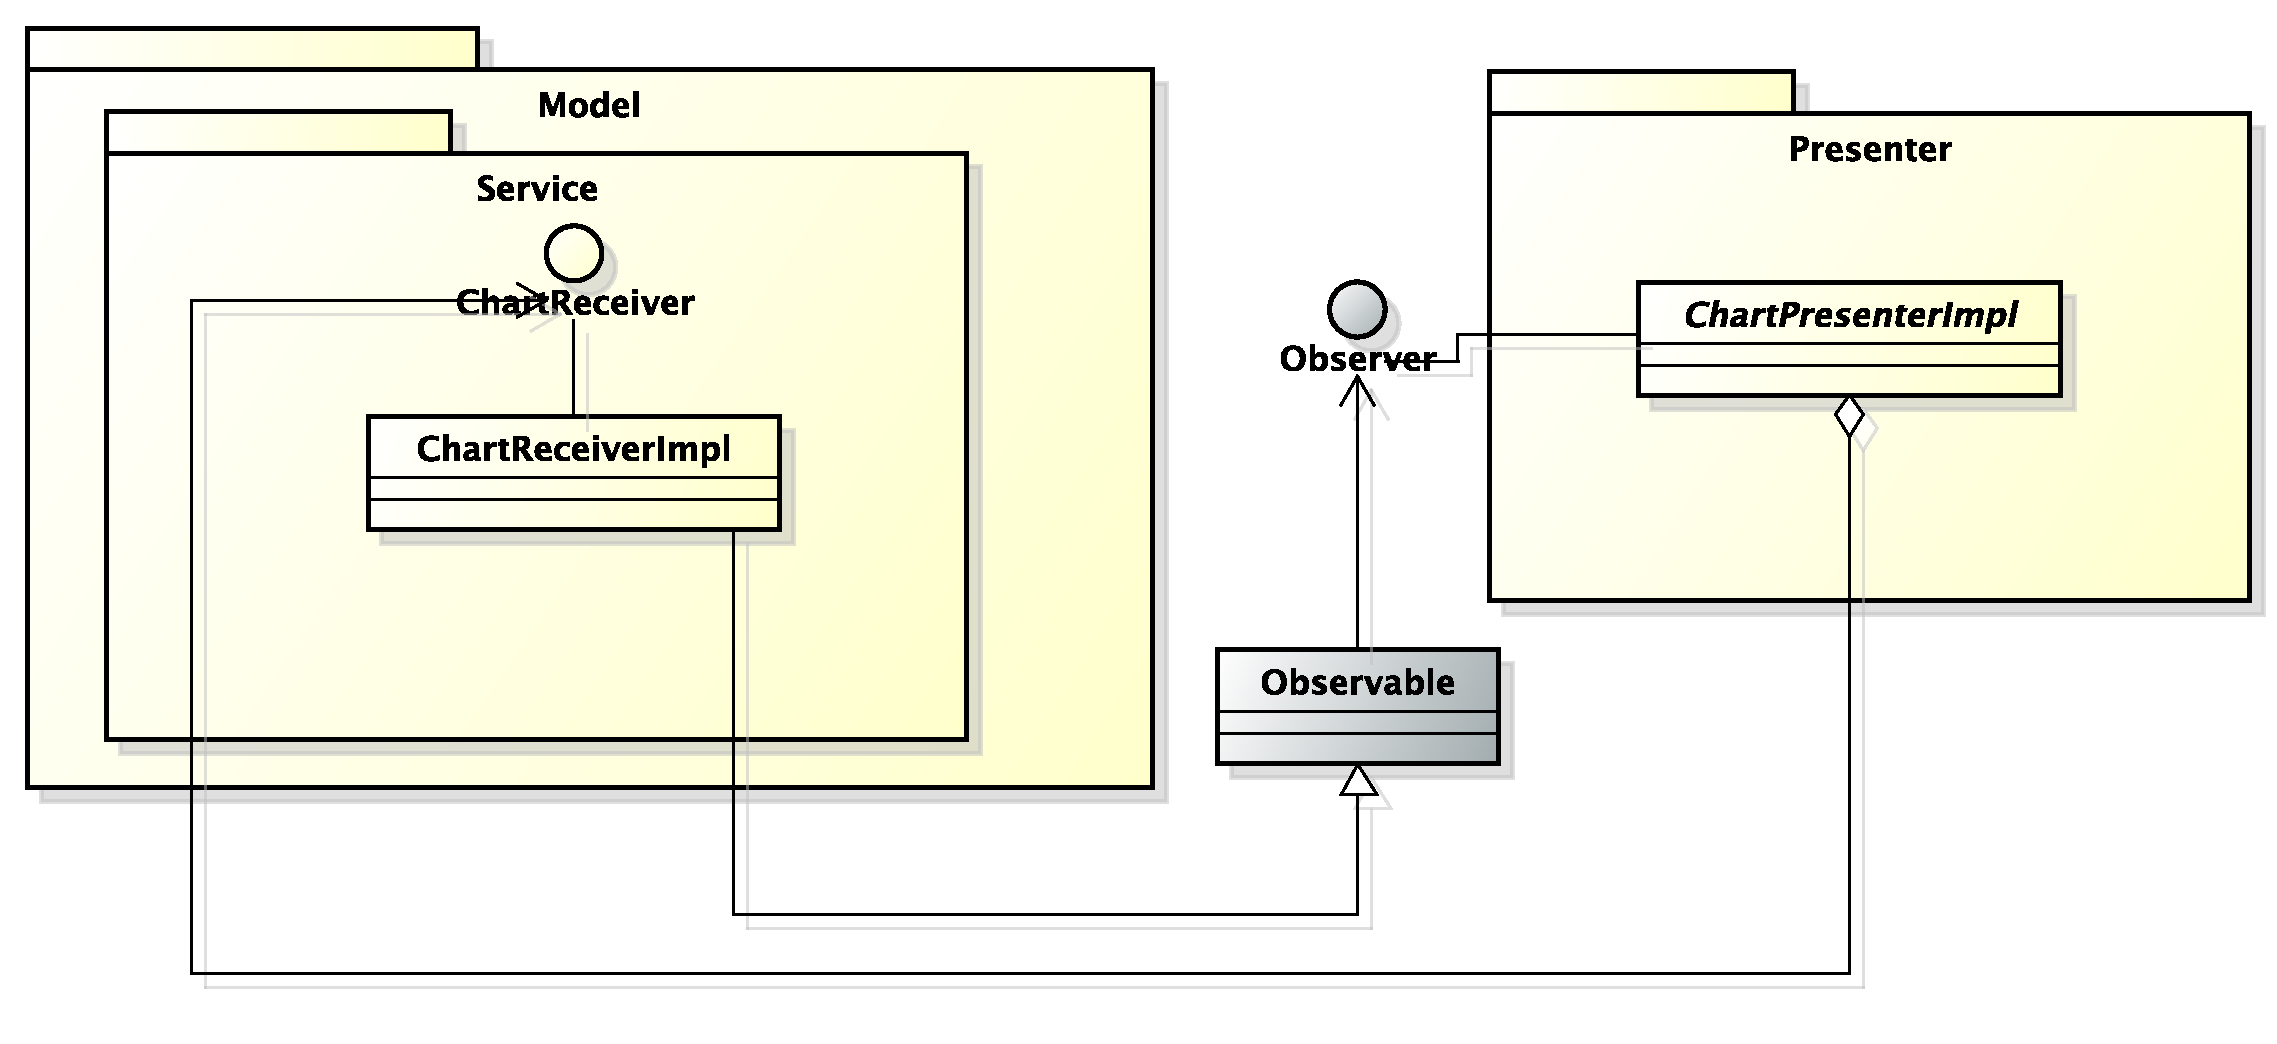
\includegraphics[width=\textwidth]{SpecificaTecnica/Pics/DesignPatternNorris/Observer}
	        		\caption{Observer pattern in Norris}
	    		\end{figure}
		
		\level{4}{Singleton}
			Il Singleton è un \insglo{pattern} creazionale il cui scopo è permettere la creazione di una sola istanza di una classe, nonchè di fornire un punto di accesso globale ad essa.\\
			Per la descrizione del \insglo{pattern} e dei vantaggi derivanti dalla sua applicazione si rimanda all'appendice \nameref{app:singleton}.
			\level{5}{Contesto di utilizzo}    		
				Le classi che implementano il Singleton sono quelle che si occupano di creare e di aggiornare i diversi tipi di grafici. Le riportiamo di seguito:
				\begin{itemize}
					\item DataModel::BarChartFactory;
					\item DataModel::LineChartFactory;
					\item DataModel::MapChartFactory;
					\item DataModel::TableFactory;
					\item DataModel::BarChartInPlaceUpdater;
					\item DataModel::LineChartInPlaceUpdater;
					\item DataModel::LineChartStreamUpdater;
					\item DataModel::MapChartInPlaceUpdater;
					\item DataModel::MapChartMovieUpdater;
					\item DataModel::TableInPlaceUpdater;
					\item DataModel::TableStreamUpdater
					\item ExternalAPIManager::ChartEndpoitFactory;
					\item ExternalAPIManager::AuthenticationEndpointFactory;
					\item ExternalAPIManager::ListEndpointFactory.
				\end{itemize}
				\begin{figure}[H]\centering
	        		\includegraphics[width=\textwidth]{SpecificaTecnica/Pics/DesignPatternNorris/Singleton1}
	        		\caption{Singleton pattern in Norris}
	    		\end{figure}
	    		\begin{figure}[H]\centering
	        		\includegraphics[width=\textwidth]{SpecificaTecnica/Pics/DesignPatternNorris/Singleton2}
	        		\caption{Singleton pattern in Norris}
	    		\end{figure}
	    		\begin{figure}[H]\centering
	        		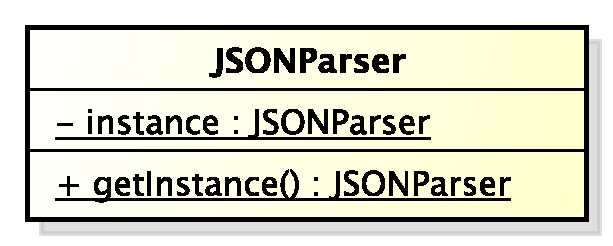
\includegraphics[width=\textwidth]{SpecificaTecnica/Pics/DesignPatternNorris/Singleton3}
	        		\caption{Singleton pattern in Norris}
	    		\end{figure}
	    		
			\level{4}{Strategy}
				\level{5}{Contesto di utilizzo}
					Le classi che implementano il Singleton sono quelle che si occupano di aggiornare i diversi tipi di grafici. Le riportiamo di seguito:
					\begin{itemize}
					\item DataModel::BarChartInPlaceUpdater;
					\item DataModel::LineChartInPlaceUpdater;
					\item DataModel::LineChartStreamUpdater;
					\item DataModel::MapChartInPlaceUpdater;
					\item DataModel::MapChartMovieUpdater;
					\item DataModel::TableInPlaceUpdater;
					\item DataModel::TableStreamUpdater
				\end{itemize}
		
